\chapter{Lecture 2 - Basics}
\section{Why visualization}
Computer-based visualization systems provide visual representations of datasets designed to help people carry on tasks more efficiently.\par
Visualization allows people to analyze data when they do not know exactly what questions they need to ask in advance. Otherwise, they can use computational techniques from statistics or learning. \par
If there are many possible questions to ask, the best path forward is an analysis process with a \emph{human in the loop}, with a visual system augmenting human capabilities, rather than replacing it.\par
Visualization allows people to offload internal cognition and memory usage to the perceptual system, using images as external representations. \par
Visualization exploits the human visual system as a mean of communication. A significant amount of visual information process occurs in parallel at the preconscious level. \par
\begin{figure}[htbp]
    \centering
    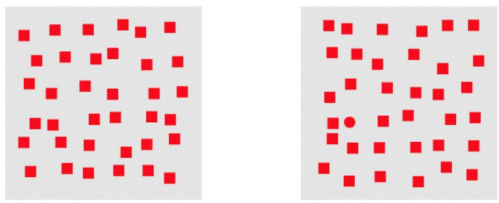
\includegraphics[width=0.3\linewidth]{imgs/lecture2/2.1 dependence on visual.png}
    \caption{Dependence on vision}
    \label{fig:2.1}
\end{figure}
Human vision can quickly find out the odd one in the fig~\ref{fig:2.1}, unlike other senses, because of the lack of parallelism in information processing.\par
\subsection{Visualization tools}
Visualization tools help people in situations where seeing the dataset structure in detail is better than seeing only a brief summary of it. \par
As the fig~\ref{fig:2.2} displays, by transforming numeric data into graphics, we can see how the data values change according to the X and Y.\par
\begin{figure}[htbp]
    \centering

    \begin{subfigure}[b]{0.32\linewidth}
        \centering
        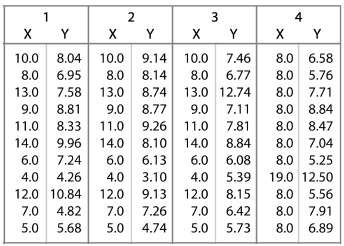
\includegraphics[width=\linewidth]{imgs/lecture2/2.2 visualization in summary.png}
        \caption{Table summary}
        \label{fig:2.2a}
    \end{subfigure}
    \hfill
    \begin{subfigure}[b]{0.32\linewidth}
        \centering
        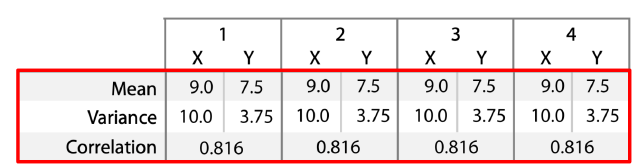
\includegraphics[width=\linewidth]{imgs/lecture2/2.3 visualizztion in detail.png}
        \caption{Table details}
        \label{fig:2.2b}
    \end{subfigure}
    \hfill
    \begin{subfigure}[b]{0.32\linewidth}
        \centering
        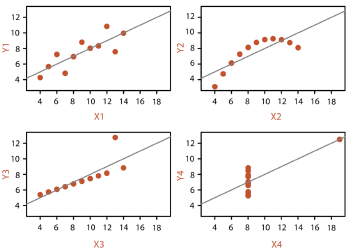
\includegraphics[width=\linewidth]{imgs/lecture2/2.4 visualization matters.png}
        \caption{Table data in graph}
        \label{fig:2.2c}
    \end{subfigure}

    \caption{Why visualization tools matter}
    \label{fig:2.2}
\end{figure}

\subsubsection{Interactivity}
Sometimes, the quantity of data is immense, and the limitations of both people and displays preclude showing everything at once. With interaction, user actions can change the view and investigate at multiple levels of detail. Look at an interactive map service, like GoogleMaps.\par

\subsubsection{Limitations}
Visualizations have limitations, especially when they come from "hardware" limitations. Human limitations are the finite resources for memory and attention. Computational capacity renders scalability a concern. And also, how the information is displayed.

\subsubsection{Task focused}
The user task is an important constraint on the visualization, as much as the data itself. \par
Visualization tools can support presentation, discovery, enjoyment of information, or even production of more information for subsequent use. A suitable visualization tool for one task is not necessarily fit for another task on the same dataset (No free lunch). Therefore, we must learn to understand which kind of visual representation to use, depending on both data and task.\par

\subsubsection{Effectiveness}
The focus on effectiveness is a corollary of defining visualization to have the goal of supporting user tasks. The goal of the designer is not to make pleasing figures but to render the results effective.\par
The vast majority of the possibilities in the design space can be ineffective in a specific usage context. This can be caused by poor design match with the properties of the human perceptual and cognitive system, or maybe it is a poor match with the intended task. 

\section{What-Why-How}
The What-Why-How method for visualization design is to answer the questions when designing the visualization.\par
\emph{What} data is being visualized? \emph{What} data are shown in the views?\par
\emph{Why} does the user need a visualization? \emph{Which} is the task being performed? \par
\emph{How} is the visual idiom constructed in terms of design choices?\par


\subsection{Semantics}
The data semantics refers to the real-world meaning of the data. As it should be provided for each dataset, as metadata. For example, the word "Apple" refers to what, the company? The fruit? the city? By means of semantics, we can take care of the ambiguity behind the data.

\section{Data Type}
The type of data is its mathematical or structural interpretation. 
There are five basic data types in visualization:
\begin{itemize}[noitemsep]
    \item \emph{Items}: an individual entity that are discrete in the dataset. They can be seen as a row in a table. 
    \item \emph{Attributes}: some specific property that can be measured, observed, or logged. In practice, they are properties of objects, also called as variables
    \item \emph{Links}: a relationship between items, typically within a network.
    \item \emph{Positions}: 2D or 3D spatial data (latitude and longitude)
    \item \emph{Grids}: they specify the strategy for sampling continuous data in terms of both geometric and topological relationships between its cells
\end{itemize}

\section{Attribute type}
The major distinction between attribute types is \emph{categorical vs ordered}. \par
\emph{Categorical} attributes are attributes whose values describe categories and do not have an implicit ordering. They can have an imposed external ordering (alphabetical order, for instance), but it is not intrinsic to the attribute itself. \par
\emph{Ordered} attributes have an implicit ordering.\par
One must choose an appropriate visual representation according to the attribute types and semantics

\subsection{Ordered attributes}
Ordered attributes can be further subdivided into:
\begin{itemize}[noitemsep]
    \item \textbf{Ordinal}: attributes which have a well-defined ordering but do not support full-pledged arithmetics (shirt size, ranking, etc.)
    \item \textbf{Quantitative}: attributes whose values represent measured quantities/magnitudes and that support arithmetic comparison (temperature, height, price, etc.)
\end{itemize}\par

Ordered attributes can have different semantics:
\begin{itemize}[noitemsep]
    \item \textbf{Sequential}: there is a homogeneous range from a minimum to a maximum value (height).
    \item \textbf{Diverging}: there are 2 sequences pointing in opposite directions that meet at a common zero-point (temperature has positive/negative value ranges).
    \item \textbf{Cyclic}: the values are wrapped around back to a starting point (hours of a day)
\end{itemize}
\section{Dataset types}
A dataset is a collection of information that is the target of analysis. The 4 basic dataset types are \emph{tables, networks, fields, and geometry}. Each of them arise from combinations of the data types of items, attributes, links, positions, and grids.\par
\begin{figure}[htbp]
    \centering
    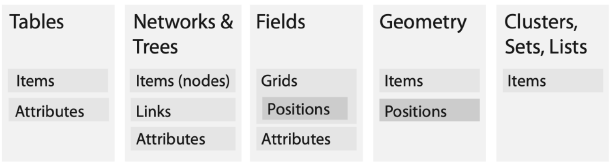
\includegraphics[width=0.5\linewidth]{imgs/lecture2/2.8 dataset types.png}
    \caption{Data and Dataset type combinations}
    \label{fig:2.6}
\end{figure}

\subsubsection{Tables}
Many datasets come in the form of tables of rows and columns, like in a spreadsheet. In a flat table, each row represents an item, and each column is an attribute of the dataset. Each cell contains a value for that pair. Multi-dimensional tables have slices and multiple keys.

\subsubsection{Networks}
Networks are suitable to specify that there is some kind of relationship between two or more items. An item in a network is called a node, and a link between 2 nodes is a relationship between two items. A network node and link can have attributes associated with them. 

\subsubsection{Trees}
Trees are networks with a hierarchical structure and no cycles. Each child node has exactly one parent node pointed to it. \par
A tree is a typical representation for hierarchy, like the organization chart of a company, or an evolutionary relationship between species in the biological tree of life.

\subsubsection{Meshes}
A 3D mesh is a particular type of graph used in computer graphics to represent 3D models. Nodes are called vertices, arcs are called edges, and there are also polygons called faces.

\subsubsection{Geometry}
They specify information about the shape of items with explicit spatial positions. 

\subsection{Fields}
Fields are a type of dataset in which values associated with a cell contain measurements or calculations from a continuous domain. Since we have a continuous domain, fields require \emph{sampling}, the measurement frequency, and \emph{interpolation}, how to show values in between the sampled points. \par
Field values are stored in grids, which have 2 properties:

\begin{itemize}[noitemsep]
    \item Geometry: position of cells in space
    \item Topology: the way cells are connected to adjacent ones
\end{itemize}

According to the values stored in cells, we can distinguish among scalar fields, vector fields, and tensor fields. These values can be static or time-dependent; deterministic or uncertain. \par

\begin{itemize}[noitemsep]
    \item \emph{Scalar} fields is one in which each cell contains a single value, for example, gray level values in medical imaging
    \item \emph{Vector} fields are ones where each cell contains a vector, represented as direction and modules (for instance, velocity)
    \item \emph{Tensor} fields are the ones where each cell contains a multi-dimensional array of attributes at each point
\end{itemize}

Continuous data is often found in the form of a spatial field, where the cell structure of the field is based on sampling at spatial positions. The data contain information about both sampled values and the position where they have been acquired.\par
According to grid geometry and grid topology, we have different types of grids: \emph{uniform, rectilinear, structured, unstructured}.

\subsubsection{Uniform grid}
They sample at a regular interval; there is no need to explicitly store topology. A uniform grid is formed of tessellations of the Euclidean plane/space by square/cubic elements, points are spaced regularly along each direction.

\subsubsection{Rectilinear grid}
They support non-uniform sampling for an efficient storage of information, at the cost of having to store geometric locations. They are useful to adapt the sampling to the geometry of the data. Its tessellations are of rectangles/rectangular cuboids, regular grids, but the spacing of points along axes can vary. They are useful to adapt the sampling to the geometry of the data. It has a fixed connectivity, yet needs to store information for spacing.

\begin{figure}[htbp]
    \centering
    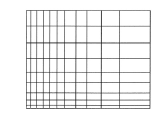
\includegraphics[width=0.2\linewidth]{imgs/lecture2/2.11 rectilinear grid.png}
    \caption{Rectilinear grid}
    \label{fig:2.9}
\end{figure}

\subsubsection{Structured grid}
They allow a curvilinear shape. It has the same connectivity as the previous two types, but an irregular geometry. Points can be replaced at an arbitrary coordinate, but no overlapping or self-intersections. It has to store the geometry of each cell.

\begin{figure}[htbp]
    \centering
    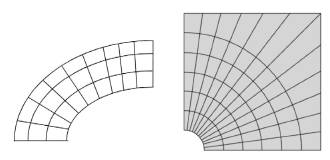
\includegraphics[width=0.2\linewidth]{imgs/lecture2/2.12 structured grid.png}
    \caption{Structured grid}
    \label{fig:2.10}
\end{figure}

\subsubsection{Unstructured grid}
They have complete flexibility, but need to store spatial positions and topological information about how the cells connect to each other. It allows different combinations of cells (a popular choice).

\begin{figure}[htbp]
    \centering
    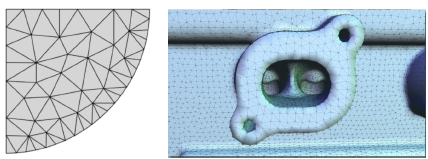
\includegraphics[width=0.25\linewidth]{imgs/lecture2/2.13 Unstructured grid.png}
    \caption{Unstructured grid}
    \label{fig:2.11}
\end{figure}

It can also be under the form of a cloud of points, but this does nor explicit any connectivity information and have irregular geometry.
